% !TEX root = ../thesis.tex
\chapter{Hardware Design}\label{cha:hardware}
The final hardware build \TODO{}

\paragraph{LED Driver}
First of all, all \glspl{LED} were directly connected to the logic wires.
This does work but the outputs of all logic \glspl{IC} have a limited current they can provide.
For example, the \emph{74LS245} is rated for maximum \qty{20}{\uA} for high-level output and \qty{-200}{\micro\ampere} for an low-level output \cite{74ls245}.
The way the \glspl{LED} were connected in the first \gls{CPU} they use only current when the logic \gls{IC} outputs a high-level voltage which is rated for \nicefrac{1}{10} the output current.
When connecting more \glspl{IC} and one \gls{LED} the maximum current can easily be exceeded.
Therefore, all \glspl{LED} of the \gls{EDiC} are powered with an additional inverting driver, the \emph{74ABT540} which is rated for \qty{50}{\uA} in both directions \cite{74abt540}.
\paragraph{Register \gls{IC}}
\begin{figure}[t]
  \centering
  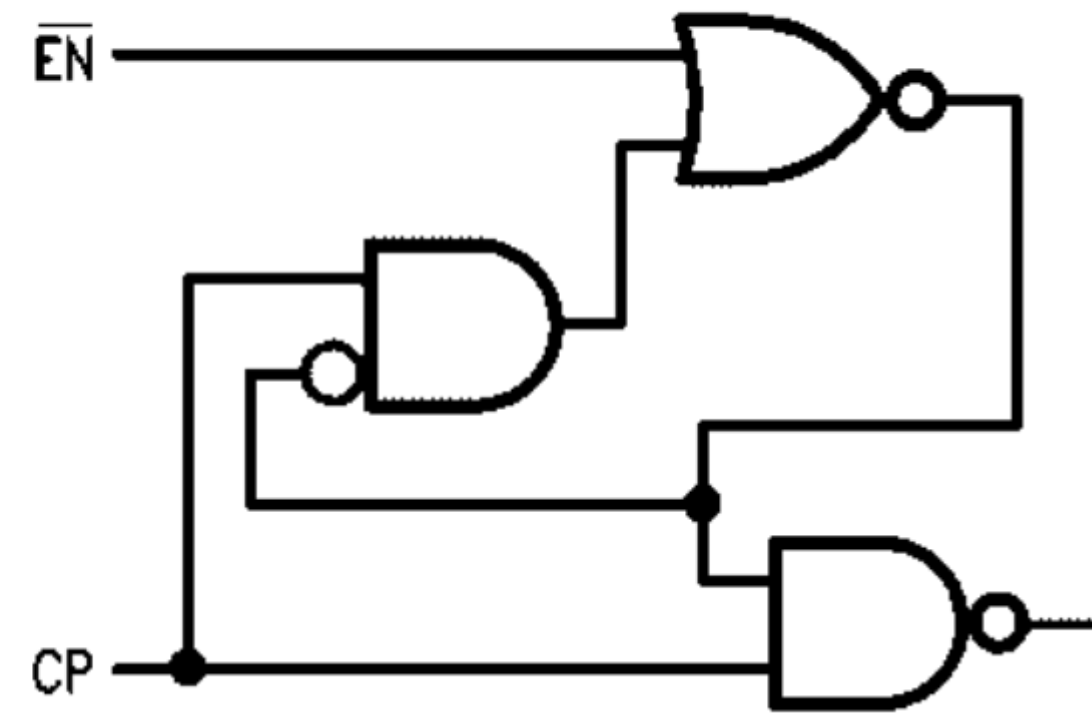
\includegraphics[width=.6\textwidth]{ce.png}
  \caption{Clock Enable circuit of the \emph{74F825} \gls{IC} \cite{74f825}.}
  \label{fig:clockEnable}
\end{figure}
% A basic 1 bit register
The 74 series of logic \glspl{IC} feature many different registers.
The most basic register \gls{IC} has $n$ D-type flip-flops with respective data inputs and outputs plus one common clock input.
On each rising edge of the clock the flip-flops capture the input values and hold them until the next rising edge of the clock.
However, often it is required that a register does not capture on every rising edge of the clock.
This is done with an additional input, called clock enable.
In the first version of the \gls{CPU} the clock inputs of the registers that needed clock enable were connected to the output of an AND gate of the clock and a control bit.
This has the major drawback that glitches of the enable control signal can propagate to the clock input of the register when the clock is currently high.
There are two widely used alternatives to the simple AND gate:
The enable input can be used as the select input for an multiplexer to the data input of the flip flop, where it multiplexes between the actual input and the current output.
This allows the flip-flop to always capture data but when the enable input is inactive, it recaptures the current output.
The drawbacks are that each bit of the register needs a multiplexer at the input and secondly that the flip-flops draw power on every clock pulse, even though no data is captured.
The \emph{74F825} logic \gls{IC} solves this with the circuit shown in \cref{fig:clockEnable}.
When the $\overline{\text{EN}}$ input is low, the CP input is NAND gate on the right passed the negated CP through\footnote{The internal flip-flops of the \emph{74F825} are negative edge triggered}.
When the $\overline{\text{EN}}$ input is high, on the other hand, the output does not change.
This circuit prevents the $\overline{\text{EN}}$ to trigger a falling edge (which would trigger the flip-flops) on the CP output.
However, when the $\overline{\text{EN}}$ goes high while the CP input is high, then the output also goes high.
This is not directly a problem because the flip-flops only trigger on falling edges but is the reason for timing requirements on the $\overline{\text{EN}}$ input which are discussed in more detail in \cref{sec:timing}.
\begin{figure}[t]
  \centering
  \begin{subfigure}[b]{.45\textwidth}
    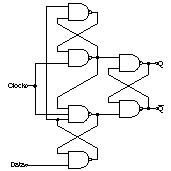
\includegraphics[height=7.5cm]{DFlipFlop.pdf}
    \subcaption{Classical D-type flip-flop built out of three $\overline{\text{SR}}$ NAND latches \cite{DFlipFlop}.}
  \end{subfigure}%
  \hspace{.05\textwidth}
  \begin{subfigure}[b]{.45\textwidth}
    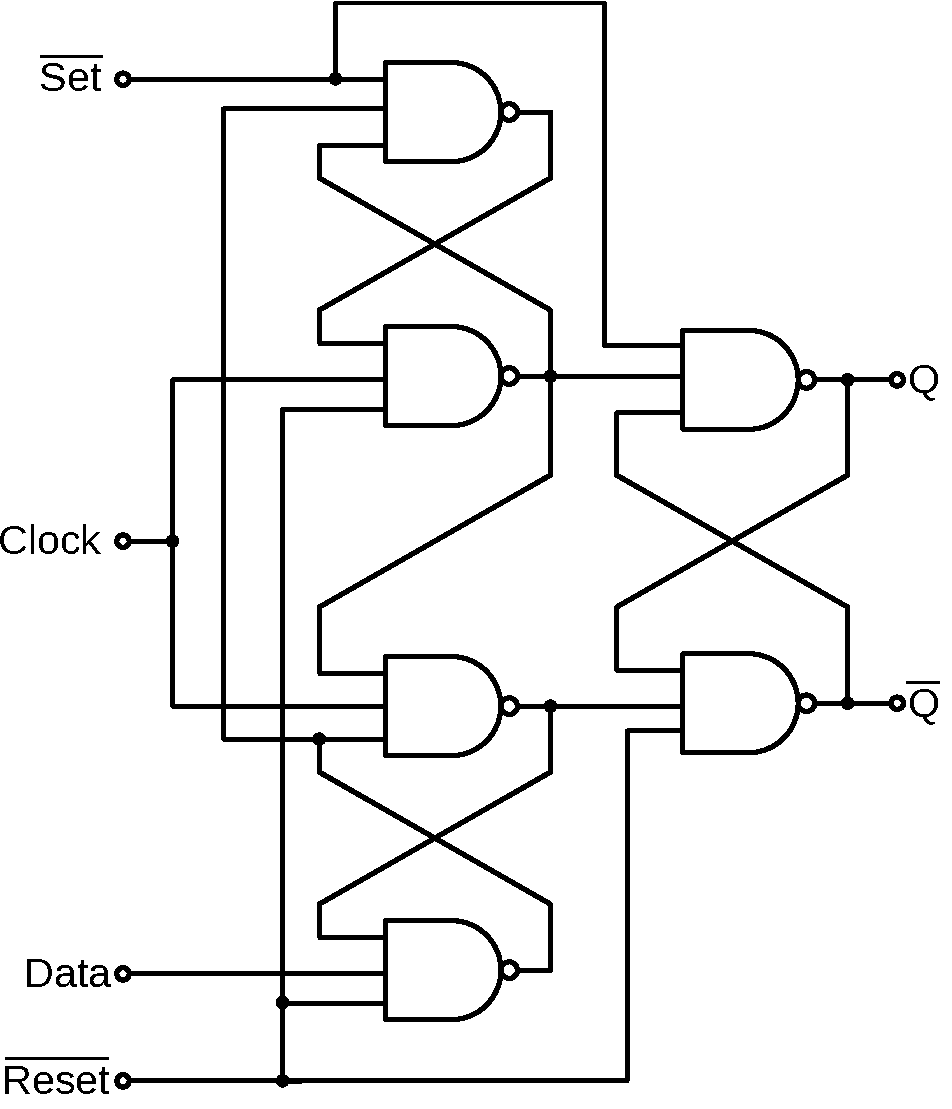
\includegraphics[height=7.5cm]{DFlipFlopClearSet.pdf}
    \subcaption{D-type flip-flop modified to support $\overline{\text{Clear}}$ and $\overline{\text{Set}}$ \cite{DFlipFlopClearSet}.}
  \end{subfigure}
  \caption{Comparison of D-type flip-flops with and without $\overline{\text{Clear}}$ and $\overline{\text{Set}}$.}
  \label{fig:clearSet}
\end{figure}
As the registers store the current state of execution, it is required that the registers start up to a known state.
Therefore, some registers feature a clear input (or set input) which forces all flip-flops to 0 (or 1).
This is usually accomplished by modifying the classical D-type flip-flop to allow for setting and resetting the internal $\overline{\text{SR}}$ NAND latches as shown in \cref{fig:clearSet}.

The third feature that may be important is a three-state output which allows the register to be directly connected to a bus.
It is accomplished by adding a tri-state output driver to the outputs of the flip-flops.

The logic \gls{IC} that was chosen for the \gls{EDiC} is the \emph{74F825} because it has all three features and is 8 bits wide.

\section{Timing Analysis}\label{sec:timing}
\begin{figure}[t]
  \centering
  \includegraphics[width=\textwidth]{timingExample.pdf}
  \caption{Timing relations for a combinatorial datapath between two registers.}
  \label{fig:timingExample}
\end{figure}
To figure out what the maximum frequency is at which the \gls{EDiC} can operate on, a detailed timing analysis was performed.
The timing analysis computes the path with the longest propagation delay which called the critical path.
The delay of the critical path can then be used as a baseline for choosing the correct frequency.

\Cref{fig:timingExample} visualizes how the propagation delays work:
Each \gls{IC} has delays which are specified in the datasheet.
In the example of \cref{fig:timingExample}, a value of register $r_0$ goes through a combinatorial path and is then stored in register $r_1$.
The registers have a propagation delay $t_p$ which specifies the time from a rising edge of the clock to the output (Q).
In theory it is also important to hold the input data of a register for the specified hold delay $t_h$, however, in the \gls{EDiC} this is no problem.
Then the combinatorial path also has propagation delays from inputs to outputs which need to be added up ($t_c$).
At the next register, a setup time $t_s$ has to be met which specifies the amount of time the input data needs to be stable before the rising edge.

\begin{figure}[t]
  \centering
  \includegraphics[width=.5\textwidth]{all_cycles.pdf}
  \caption{Timing analysis for the control signals.}
  \label{fig:timingControl}
\end{figure}
The \cref{fig:timingControl,fig:timingRam,fig:timingAlu} show three timing analysis for the \gls{EDiC}.
Each block represents one \gls{IC} with the corresponding delay.
The first column shows the unit number of the schematic, the second line the type of \gls{IC} and the third shows the kind of delay with the fourth showing the time.
The kind of delay of a buffer can for example be d$\rightarrow$ q which means input data to output data delay or oe$\rightarrow$ q which is the time from asserting output enable until the data is valid.
The delay time is always the worst case time as specified in the datasheet\footnote{Propagation typically vary with the temperature and age of the \gls{IC} and by taking the worst case time (maximum) it is assured that no timings bugs occur due to e.g. weather changes.}.
A vertical double line represents a point where multiple delay paths must be met until the execution can continue.
In \cref{fig:timingControl} for example, the propagation delay of register U83 (flags and step register) and register U84 (instruction) must both be over until the address for the \glspl{EEPROM} U85, U86 and U87 are valid.
At these points the maximum of the merging delay paths is used as the starting point for the next path.
The maximum delay up to this point is also added at the top.
Additionally, some paths are labeled for clarity.
All the times of the critical path (the path that takes the longest from one starting point to one end point) are marked in red.

\twopagepicture{t}{p}{ram.pdf}{Timing analysis for the memory latency.}{fig:timingRam}
\twopagepicture{t}{p}{alu.pdf}{Timing analysis for the \gls{ALU} latency.}{fig:timingAlu}